\documentclass[mathserif]{beamer}
\usetheme{Berkeley}
\usecolortheme{albatross}
\usepackage{listings}

\title{Constructing a Knowledge Base on Aging}
\subtitle{An Automated Approach}
\author{Mark Farrell}
\institute
{

Bioinformatics Researcher \and

\inst{}%
Center for Research and Education on Aging \\
Lawrence Berkeley National Laboratory \\
University of California, Berkeley

}

\date{September 4th, 2014}
\subject{Natural Language Processing}

\AtBeginSection[]
{
\begin{frame}
\frametitle{Outline}
\tableofcontents[currentsection]
\end{frame}
}

\lstset{
basicstyle=\small\sffamily,
columns=fullflexible,
showstringspaces=false
}

\begin{document}

\frame{\titlepage}

\section{Automatically Constructing Knowledge Bases}

\begin{frame}

\frametitle{Overview}

\begin{itemize}[<+->]

\item CREA is constructing a knowledge base to study and
understand the human aging process.
\item New discoveries are published quickly and in large
volume.
\item It is infeasible to construct the knowledge base by
hand.
\item Working on software to construct the knowledge base
automatically.

\end{itemize}

\end{frame}

\begin{frame}

\frametitle{Introduction}
\framesubtitle{How to Automatically Construct the Knowledge Base}

\begin{itemize}[<+->]

\item Routinely search for keywords related to aging, dowloading
text articles from sources like PubMed and WebMD.
\item Build a spam filter to get rid of non-scientific sentences.
\item Extract scientific facts from the sentences and save them
in a structured format.
\item Provide a graphical interface that allows users to search
and otherwise explore the knowledge base.

\end{itemize}

\end{frame}

\begin{frame}

\frametitle{Summary of Progress}

\begin{itemize}[<+->]

\item Devised and implemented the method for finding simple facts
in sentences, extracting them in a structured format.

% Projects like Carnegie Mellon's "Read The Web" appear to be able
% to extract simple facts from sentences, but their software is
% neither open-source nor downloadable.

\item Began work on a web viewer for the knowledge base.

\end{itemize}

\end{frame}

\section{Extracting Facts in a Structured Format}

\begin{frame}

\frametitle{Tokenization}

\begin{itemize}[<+->]

\item Input a text document and read it, one sentence at a time.

\end{itemize}

\end{frame}

\begin{frame}[fragile]


\begin{block}{Example: Tokenization}
\begin{lstlisting}
scala> tokens("The man walks. The dog eats.")
res0: List[String] = List(The man walks., The dog eats.)
\end{lstlisting}
\end{block}

\end{frame}

\begin{frame}

\frametitle{Parsing}

\begin{itemize}[<+->]

\item For each sentence, generate a constituent tree that describes its phrase structure.

\end{itemize}

\end{frame}

\begin{frame}[fragile]

\begin{block}{Example: Parsing}
\begin{lstlisting}
scala> parse("The man walks the dog.")
res0: Tree[String] = (ROOT
  (S
    (@S
      (NP (DT The) (NN man))
      (VP (VBZ walks)
        (NP (DT the) (NN dog))))
    (. .)))
\end{lstlisting}
\end{block}

\end{frame}

\begin{frame}

\frametitle{Parsing Method}

\begin{itemize}[<+->]

\item The University of Pennsylvania Treebank Project:
\begin{itemize}[<+->]

\item Defines notation for constituent trees.
\item Parses sentences from the Wall Street Journal by hand.

\end{itemize}

\item The Berkeley Parser is software that guesses how to parse a sentence from the notation and examples specified by the Penn Treebank.

\end{itemize}

\end{frame}

\begin{frame}

\frametitle{Compilation}

\begin{itemize}[<+->]

\item Extract facts from each constituent tree.

\end{itemize}

\end{frame}

\begin{frame}[fragile]

% In this example, the man is the subject and the dog is the object.
\begin{block}{Example: Compilation}
\begin{lstlisting}
scala> compile("The man walks the dog.").shows
res0: String = [<compound:walk(<atom:man>, <atom:dog>)>]
\end{lstlisting}
\end{block}

\end{frame}

\begin{frame}

\frametitle{Compilation Method}

Pattern match on the constituent trees. Define patterns for:

\begin{enumerate}[<+->]

\item Extracting nouns from noun phrases (NP).
\item Extracting predicates and nouns from verb phrases (VP).
\item Extracting facts from complete clauses (S), making logical
assertions with nouns and predicates.

\end{enumerate}

\end{frame}


\section{Results \& Discussion}

\begin{frame}

\frametitle{Software Demonstration}
\framesubtitle{A preview of CREA's knowledge base, compiled from
PubMed abstracts.}

\href{http://markfarrell.ca/creal}{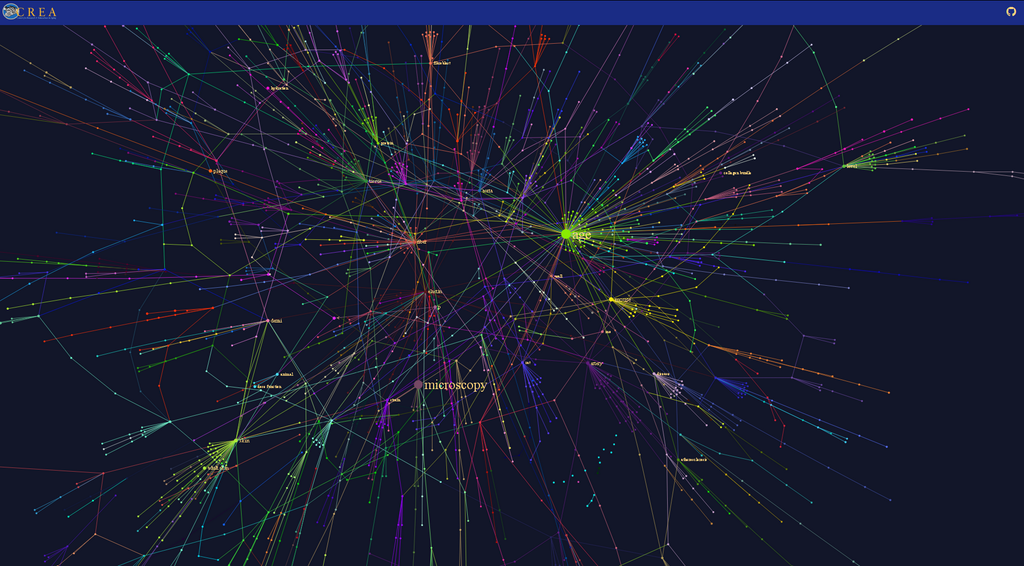
\includegraphics[width=1.0\linewidth]{results.png}}

\end{frame}

\begin{frame}

\frametitle{Performance}
\framesubtitle{Parallelization}

\begin{itemize}[<+->]

\item It is possible to extract facts from many sentences at the same time.

\end{itemize}

\end{frame}

\begin{frame}

\frametitle{Accuracy}

\begin{itemize}[<+->]

\item Filter spam sentences from documents.

\item The accuracy of the parser could be optimized:
\begin{itemize}[<+->]

\item Should be trained to identify more nouns from the biomedical
domain.

\end{itemize}

\item Define more patterns for extracting facts:
\begin{itemize}[<+->]

\item The software succeeds around 50\% of the time.

\end{itemize}

\end{itemize}

\end{frame}

\begin{frame}

\frametitle{Missing Features}

\begin{itemize}[<+->]

\item Support negated clauses and conditional logic.

\item Facts can contradict each other:
\begin{itemize}[<+->]
\item Store the probability that is true as the weight of its edge on the
knowledge base's graph.
\end{itemize}

\item Scale and launch the software service.

\end{itemize}

\end{frame}

\begin{frame}

\frametitle{Conclusion}

\begin{itemize}[<+->]

\item Demonstrated a method for automatically constructing CREA's
knowledge base on aging.
\item Showed how to extract facts from English text in the knowledge
base's structured format.
\item Discussed the need to improve software accuracy by lensing in on
the biomedical domain.
\item Suggested how the software implementation can be scaled for
production usage.

\end{itemize}

\end{frame}

\end{document}
